%-----Main FIle------

\documentclass[10pt,a4paper]{report}

%adjust your page margins here
\usepackage[top=0.70in, bottom=0.70in, left=0.8in,right=0.80in]{geometry} % setting the page alignment with this package
\usepackage{graphicx} % for embedding images
% \usepackage[hyphens]{url} % for proper url entries
\usepackage{hyperref} % for creating links in the pdf version and other additional pdf attributes, no effect on the printed document
\usepackage{float} % used for figure placement with H as a parameter
\usepackage{subcaption}
% \usepackage[hyphens]{url}
% \usepackage{hyperref}
\usepackage{mathptmx} % for Times New Roman; pslatex is obsolete
\usepackage{amsmath}
\usepackage{array} % for making text bold in table
\usepackage{url} % for URL formatting
\hypersetup{
    colorlinks=true,
    linkcolor=blue,
    filecolor=magenta,      
    urlcolor=cyan,
}


%For inserting Python Code
\usepackage{listings}
\usepackage{color}
 
\definecolor{dkgreen}{rgb}{0,0.6,0}
\definecolor{gray}{rgb}{0.5,0.5,0.5}
\definecolor{mauve}{rgb}{0.58,0,0.82}
 
\lstset{ %
  language=Python,                % the language of the code
  basicstyle=\footnotesize,           % the size of the fonts that are used for the code
  numbers=left,                   % where to put the line-numbers
  numberstyle=\tiny\color{gray},  % the style that is used for the line-numbers
  stepnumber=1,                   % each line is numbered
  numbersep=5pt,                  % how far the line-numbers are from the code
  showspaces=false,               % show spaces adding particular underscores
  showstringspaces=false,         % underline spaces within strings
  showtabs=false,                 % show tabs within strings adding particular underscores
  frame=single,                   % adds a frame around the code
  rulecolor=\color{black},        % if not set, the frame-color may be changed on line-breaks within not-black text (e.g. commens (green here))
  tabsize=2,                      % sets default tabsize to 2 spaces
  captionpos=b,                   % sets the caption-position to bottom
  breaklines=true,                % sets automatic line breaking
  breakatwhitespace=true,        % sets if automatic breaks should only happen at whitespace
  title=\lstname,                   % show the filename of files included with \lstinputlisting;
                                  % also try caption instead of title
  keywordstyle=\color{blue},          % keyword style
  commentstyle=\color{dkgreen},       % comment style
  stringstyle=\color{mauve},         % string literal style
  escapeinside={\%*}{*)},            % if you want to add a comment within your code
  morekeywords={*,...}               % if you want to add more keywords to the set
}
%For inserting Python Code Over


% For the header and footer start
\usepackage{fancyhdr}

% Define the default page style
\fancypagestyle{plain}{%
  \fancyhf{} % Clear all header and footer fields
  \fancyfoot[L]{\emph{This project implements multiple source detection techniques on different networks}} % Left footer
  \fancyfoot[R]{\thepage} % Right footer
  \renewcommand{\headrulewidth}{0pt} % No header line
  \renewcommand{\footrulewidth}{0.4pt} % Footer line
}

% Applying the page style
\pagestyle{fancy}
\fancyhf{} % Clear all header and footer fields for the fancy style

% Define the headers
\fancyhead[L]{Chapter \thechapter} % Left header
\renewcommand{\chaptermark}[1]{\markboth{#1}{}}
% For the header and footer over


%GLOBAL SETTINGS OVER, DOCUMENT BEGINS
\begin{document}

%FROM HERE YOUR PAGES START GETTING ADDED

% includes the cover page
%-----------------------------------------------------------------------------------
%   TITLE PAGE
%-----------------------------------------------------------------------------------
\begin{titlepage}

\newcommand{\HRule}{\rule{\linewidth}{0.5mm}} % Defines a new command for horizontal lines, change thickness here

\center % Center everything on the page

%-----------------------------------------------------------------------------------
%   HEADING SECTIONS
%-----------------------------------------------------------------------------------
\textsc{\LARGE École Polytechnique Fédérale de Lausanne}\\[2cm] % University name
\textsc{\Large Research Project}\\[1cm] % Course code and name
\textsc{\large Bachelor's Thesis}\\[1.2cm] % Project type

%-----------------------------------------------------------------------------------
%   TITLE SECTION
%-----------------------------------------------------------------------------------
\HRule \\[0.8cm]
{ \huge \bfseries Simulation and Source Detection of Infectious Processes on Networks}\\[0.4cm] % Document title
\HRule \\[2cm]
 
%-----------------------------------------------------------------------------------
%   AUTHOR SECTION
%-----------------------------------------------------------------------------------
\begin{minipage}{0.4\textwidth}
\begin{flushleft} \large
\emph{Author:}\\
Ahmed Abdelmalek\\
\end{flushleft}
\end{minipage}
~
\begin{minipage}{0.4\textwidth}
\begin{flushright} \large
\emph{Supervisor:} \\
Paula Murmann
\end{flushright}
\end{minipage}\\[2cm]

%-----------------------------------------------------------------------------------
%   DATE SECTION
%-----------------------------------------------------------------------------------
{\large \today}\\[2cm]

%-----------------------------------------------------------------------------------
%   LOGO AND ADDRESS SECTIONS
%-----------------------------------------------------------------------------------
\begin{minipage}[t]{0.5\textwidth}
    \centering
    
\includegraphics[width=0.8\linewidth]{logo_epfl.png}\\[0.5cm]
    \textit{School of Computer and Communication Sciences}\\
    \textit{École Polytechnique Fédérale de Lausanne}\\
    \textit{Route Cantonale}\\
    \textit{CH-1015 Lausanne, Switzerland}
\end{minipage}%
\begin{minipage}[t]{0.5\textwidth}
    \centering
    
\includegraphics[width=0.8\linewidth]{logo_indy_lab.png}\\[0.5cm]
    \textit{Information and Network Dynamics Lab}\\
    \textit{EPFL IC IINFCOM INDY 2}\\
    \textit{Station 14}\\
    \textit{CH-1015 Lausanne, Switzerland}
\end{minipage}

\vfill % Fill the rest of the page with whitespace

\end{titlepage}
 
\newpage

% includes the dedication page
%-----------------------------------------------------------------------------------
%   DEDICATION PAGE
%-----------------------------------------------------------------------------------

\thispagestyle{empty} % Ensures no headers or footers are used on this page
\begin{center}
    \vspace*{\fill} % Vertically centers the content on the page
    \textit{"At least I tried"}\\[0.5cm]
    --- Ann Brashares\\[3cm]

    Dedicated to the curious side of me that drives me crazy.\\[0.5cm]
    And to my idolized grandfather, who showered me with his fountain of knowledge.
    \vspace*{\fill}
\end{center}

\newpage

% includes the acknowledgements page
%-----------------------------------------------------------------------------------
%   ACKNOWLEDGEMENTS PAGE
%-----------------------------------------------------------------------------------

\thispagestyle{empty} % Removes the page number on this page
\begin{center}
    \Large \textbf{Acknowledgements}\\[2cm]
\end{center}

\linespread{1.3}\selectfont % Adjust line spacing for the acknowledgement section and apply it

\noindent
I am grateful to Paula Murmann for her guidance throughout the entire semester. Her expertise has significantly shaped this project.\\

\noindent
I am also thankful to my parents, who have provided emotional support throughout my bachelor studies. Their encouragement has been my foundation, and I owe them my heartfelt recognition.\\

\noindent
Lastly, a hat tip to all the professors of the IC faculty who transmitted their knowledge and their passion for this domain.\\[2cm]

\hfill Ahmed Abdelmalek % Right-aligned name at the bottom 
\newpage

% includes the abstract page
\begin{center}
    \thispagestyle{empty} % Removes the page number on this page
    \Large \textbf{ABSTRACT}\\[2cm]
\end{center}

\noindent
This project explores the simulation of infectious processes on networks, focusing on the identification of infection sources within grids then graph-based models. We first go through the implementation of some grid-based algorithms and then their comparison using different criteria, then we move to networks and we compare our algorithms outcomes to other literature's results. Although in a grid-based homogeneous infection, it would be a lot easier to find the source of the infection, results indicate that certain network structures enhance the traceability of the infection origin, offering potential strategies for effective disease monitoring and control. This project contributes to our understanding of infections' spread, and how would the model affect the source detection of the infection.
\newpage

%TABLE OF CONTENTS AND LIST OF FIGURES ARE AUTOMATICALLY ADDED BY FOLLOWING COMMANDS
%ADD FIGURE OF TABLES IF YOU NEED TO, CHECK DOCUMENTATION
\pagenumbering{roman} %numbering before main content starts


%To reset the Header & Footer for TOC and LOF
\pagestyle{empty}
\addtocontents{toc}{\protect\thispagestyle{empty}}
\tableofcontents % adds Index Page

%\pagestyle{empty}

\addtocontents{lof}{\protect\thispagestyle{empty}}
\listoffigures % adds List of Figures
\cleardoublepage

%And reset back the settings we choose for Header and Footer
\pagestyle{fancy}

\newpage
\pagenumbering{arabic} %reset numbering to normal for the main content

\chapter{Introduction}
Infectious diseases necessitate robust models to simulate their spread. Network analysis serves as a powerful tool in this domain, enabling researchers to visualize and predict how diseases propagate through communities. This project utilizes grid-based and network-based simulations to explore the dynamics of disease spread, employing various structures to mirror the complexity of real-world interactions.

\section{Main Challenges}
One of the main challenges in this research is the identification of the source of an infection within a network. This task is particularly daunting due to the diverse and complex nature of network structures, which can significantly affect the propagation paths of infectious agents.

\section{Limitations}
Existing models like the SIR and SIS, while foundational, often fall short in capturing phenomena such as waning immunity and recurrent infections, which are critical for understanding diseases like COVID-19.

\section{Introduction to the SIRS Model}
The SIRS model addresses these shortcomings by incorporating waning immunity, making it particularly relevant for diseases that do not confer lifelong immunity. This model forms the cornerstone of our study.

\begin{figure}[H]
    \centering
    \includegraphics[width=0.8\textwidth]{SIRS_Model_Dynamics.png}
    \caption{SIRS model dynamics}
    \label{fig:SIRS_Model_Dynamics}
\end{figure}

\section{Approach}
Our approach integrates simulating an infectious disease on both grid-based and graph-based models, then applying our source recovery detection algorithms. We will employ various centrality measures to enhance the accuracy of source identification. The goal is to have a clear success rate of infection source recovery over time and to understand the underlying reasons for these results. This allows for a comprehensive analysis of infection dynamics, accommodating the distinct features of each network type. The integration of multiple network models and centrality measures is essential for developing a nuanced understanding of disease spread.

\section{Thesis Statement}
Our comparative study shows a marked improvement in source detection within both fixed and non-fixed boundary conditions for a grid-based model and how these source detection algorithms work on other network models. The core contribution of this thesis lies in its development of a simulation framework that adapts to various network structures, enhancing the accuracy of source detection. This advancement not only improves our theoretical understanding of network-based disease spread but also has practical implications for designing more effective containment measures. % adds the introduction page
\chapter{Literature Review}

\section{A Historical Perspective on Identifying Propagation Sources in Networks}
For decades, researchers have been captivated by the challenge of identifying propagation sources within networks, a quest that extends across diverse domains, from managing disease outbreaks in biological networks to tracking the genesis of rumors across social media platforms. This introduction sets out to explore the evolutionary trajectory of methodologies used to address this pivotal challenge.\\

Early approaches focused on leveraging \textbf{centrality measures} within network structures, as explored by Granovetter \cite{granovetter1973}. These pioneering works investigated concepts like Degree Centrality, Closeness Centrality, Betweenness Centrality, and Eigenvector Centrality to identify influential nodes within a network. Nodes with high centrality scores were considered potential sources of propagation.\\

However, as network research matured, limitations of centrality measures became apparent. Researchers turned to more sophisticated approaches that incorporated information about the underlying propagation processes. Statistical methods emerged, capitalizing on the \textbf{temporal dynamics} of propagation \cite{liu2011, chen2010}. These methods exploited the fact that information typically spreads outward from the source, allowing for inferences based on the timing and directionality of propagation events.\\

The rise of \textbf{complex network theory} further diversified source identification methodologies. Researchers recognized the intricate structures of real-world networks, such as community structures and varying node degrees. Works by Zhou et al. \cite{zhou2008} and Gomez-Rodriguez et al. \cite{gomez2011} explored leveraging these features for improved source identification accuracy. Their approaches incorporated information about community memberships and node connectivity patterns to refine the search for potential sources.\\

The landscape continues to evolve. Recently, researchers have begun integrating \textbf{machine learning} and \textbf{data-driven techniques}. Studies by Zhao et al. \cite{zhao2016} and Gao et al. \cite{gao2018} explored the use of supervised learning algorithms to predict the source of propagation events based on historical data. These methods offer promising results in specific scenarios but often require access to large datasets for effective training.\\

This literature review builds upon this rich history, exploring the strengths and limitations of existing methodologies for source identification in networks. By examining various approaches across different studies \cite{wang2020, shelke2019, doe2018, liu2020}, we aim to identify areas for improvement and pave the way for the development of more robust and adaptable source identification techniques. Ultimately, this pursuit holds significant implications for understanding and potentially controlling various processes unfolding within complex networks.

\section{Methodologies in Propagation Source Identification}
\subsection{Centrality Measures in Source Detection}
This extensive review by Wang et al. \cite{wang2020} explores a broad spectrum of centrality measures, including Degree Centrality, Closeness Centrality, Betweenness Centrality, and Eigenvector Centrality. They evaluate the applicability and effectiveness of these measures for source detection within various network structures. Their work provides a comprehensive understanding of how different centrality measures perform in identifying the origin of propagation across diverse network types.

\subsection{Taxonomy of Source Detection Techniques}
Shelke \& Attar \cite{shelke2019} offer a structured taxonomy that categorizes source detection techniques into three main categories: structural, diffusion-based, and probabilistic approaches. Their methodology emphasizes the role of network features such as topology (network structure) and dynamics (how information or disease spreads over time) in determining the accuracy of source detection. This categorization helps us understand how different techniques leverage network properties to pinpoint the source of propagation.

\subsection{Centrality Measures for Infection Source Identification}
Doe et al. \cite{doe2018} investigate the use of classical graph centrality measures specifically for identifying infection sources. They employ a range of measures, including Degree, Betweenness, Closeness, and Eigenvector Centrality, to assess their performance across different network structures. Their work sheds light on the variability in performance of these centrality measures depending on network characteristics. This knowledge informs our selection of appropriate centrality measures for source identification within our chosen network models (grid-based and graph-based).

\subsection{Stochastic Modeling of Epidemic Spread}
While the previous studies focused on network analysis techniques, Liu et al. \cite{liu2020} introduce a novel approach using stochastic modeling. They propose a stochastic SIRS epidemic model that incorporates logistic growth and stochastic perturbations. Their methodology involves developing stochastic differential equations (SDEs) to model disease dynamics. By evaluating the impact of stochastic perturbations (random variations) on epidemic spread, this work highlights the inherent randomness present in real-world outbreaks.\\

The methodologies employed in these studies showcase the multifaceted approach needed for identifying propagation sources in networks, enriching the field with diverse perspectives.

\section{Key Findings and Insights}
Across these studies, several key findings emerge. Wang et al. \cite{wang2020} demonstrated that integrating multiple centrality measures improves source detection accuracy in networks. They found that specific combinations like Closeness Centrality and Eigenvector Centrality are particularly effective in pinpointing the origin of spread. Shelke \& Attar \cite{shelke2019} emphasized the effectiveness of structural methods for static networks, while diffusion-based methods perform better in dynamic environments. Doe et al. \cite{doe2018} highlighted the variability in centrality measure performance across different network structures, underscoring the need for careful selection based on network characteristics. Finally, Liu et al. \cite{liu2020} illustrated the significant impact of stochastic perturbations on epidemic dynamics. Their work highlighted the role of stochasticity in shaping the long-term behavior of epidemics, affecting their persistence and stability. These findings contribute to a deeper understanding of infection source detection in networks and emphasize the complex interplay between network structure, dynamics, and stochasticity.

\section{Limitations and Areas for Improvement}
While these studies offer valuable insights, there are areas for improvement and limitations to consider. Wang et al. \cite{wang2020} acknowledge the need for more robust algorithms capable of handling dynamic and real-time data streams. Additionally, they highlight the importance of integrating probabilistic models to account for uncertainties inherent in network propagation. Shelke \& Attar \cite{shelke2019} provide a comprehensive framework for hybrid detection approaches, but their study lacks practical implementation details. Doe et al. \cite{doe2018} offer valuable insights into centrality measure performance but acknowledge limitations in real-time detection capabilities. Finally, Liu et al. \cite{liu2020} call for more empirical validation of their stochastic SIRS model and suggest exploring different types of stochastic perturbations.\\

Despite these limitations, these studies collectively advance the understanding of infection source detection in networks. They offer valuable insights into the selection of centrality measures and hybrid approaches, contribute to the development of simulation frameworks, and enhance the accuracy of infection spread models. Moreover, they highlight the importance of considering network structure, dynamics, and stochasticity when understanding disease spread in networks \cite{wang2020, shelke2019, doe2018, liu2020}.

\section{Use for the Thesis and Main Contribution to the Field}
\subsection{Use for the Thesis}
The methodologies and findings from these studies directly inform the thesis, providing guidance on the selection of centrality measures and hybrid approaches for infection source detection. They contribute to the development of simulation frameworks and enhance the accuracy of infection spread models. The insights gleaned from these papers and books enrich the understanding of disease dynamics in networked environments, facilitating the design of more effective containment measures and intervention strategies. Additionally, they offer valuable perspectives on the complex interplay between network structure, dynamics, and stochasticity in shaping disease spread, providing a solid foundation for further research in the field.\\

By examining the strengths and limitations of these methods \cite{wang2020, shelke2019, doe2018, liu2020}, we aim to lay the groundwork for a comprehensive framework for source identification within the context of our research project.

\subsection{Main Contribution to the Field}
The insights gleaned from this review inform the core of our project – investigating disease spread across different network structures. By integrating established centrality measures with potentially more nuanced approaches, we aim to develop a robust framework for source identification within both grid-based and graph-based network models. This project contributes to the field by:
\begin{itemize}
    \item \textbf{Enhancing source identification accuracy}: By leveraging a combination of established and potentially more tailored methods, we aim to achieve a higher success rate in pinpointing infection sources compared to existing approaches that rely on singular techniques.
    \item \textbf{Understanding the interplay between network structure and source identification}: Our comparative study across grid-based and graph-based models will illuminate how network characteristics influence the effectiveness of different source identification algorithms. This knowledge will contribute to the development of more adaptable frameworks that can be tailored to specific network types.
    \item \textbf{Informing disease containment strategies}: Improved source identification accuracy translates to faster intervention and containment measures. By providing a more comprehensive understanding of source detection within different network structures, this project has the potential to inform the development of more effective disease control strategies.
\end{itemize}

\section{Conclusion}
The reviewed studies showcase the multifaceted approach needed for identifying propagation sources in networks. They offer valuable insights into the selection of centrality measures, hybrid approaches, and the development of simulation frameworks to enhance the accuracy of infection spread models. % adds the literature-review page
\chapter{Mathematical Modeling}

Understanding the spread of infectious diseases in complex networks is critical for effective epidemic control \cite{hellewell2020, britton2021}. Network theory provides valuable insights into how diseases propagate through populations \cite{newman2010}, and centrality measures play a crucial role in identifying influential spreaders and potential epidemic sources \cite{gomez2011}.

This chapter provides the foundational knowledge necessary for modeling infectious diseases, focusing on one key model: \textbf{SIRS}. We will discuss the differential equations governing this model and methods to quantify the speed of infection.

\section{Mathematical Modeling of an SIRS process}
Infectious diseases can be modeled using differential equations that describe the changes in the number of susceptible (S), infected (I), and recovered (R) individuals over time.\\
\noindent
The SIRS model includes a return to susceptibility after recovery, accounting for waning immunity. The compartments are:
\begin{itemize}
    \item \textbf{Susceptible (S):} Individuals who can contract the disease.
    \item \textbf{Infected (I):} Individuals who have contracted the disease and can transmit it.
    \item \textbf{Recovered (R):} Individuals who have recovered from the disease but can become susceptible again.
\end{itemize}

\begin{figure}[H]
    \centering
    \includegraphics[width=0.9\textwidth]{img/SIRS_Model_Dynamics.png}
    \caption{SIRS model dynamics}
    \label{fig:SIRS_Model_Dynamics}
\end{figure}

\noindent
The differential equations for the SIRS model are \cite{hethcote2000, anderson1992}:
\begin{equation}
\frac{dS}{dt} = \delta R - \beta SI,
\label{equation:3.1}
\end{equation}
\begin{equation}
\frac{dI}{dt} = \beta SI - \gamma I,
\label{equation:3.2}
\end{equation}
\begin{equation}
\frac{dR}{dt} = \gamma I - \delta R,
\label{equation:3.3}
\end{equation}

where $\beta$ is the infection rate, $\gamma$ is the recovery rate, and $\delta$ is the rate at which recovered individuals become susceptible again.\\

\noindent
To capture the inherent randomness in disease spread, the stochastic version of the model can be represented using stochastic differential equations (SDEs) \cite{liu2020, jiang2017}:

\begin{equation}
dS = \left(\delta R - \beta SI\right) \, dt + \sigma_S \, S \, dW_S,
\label{equation:3.4}
\end{equation}

\begin{equation}
dI = \left(\beta SI - \gamma I\right) \, dt + \sigma_I \, I \, dW_I,
\label{equation:3.5}
\end{equation}

\begin{equation}
dR = \left(\gamma I - \delta R\right) \, dt + \sigma_R \, R \, dW_R,
\label{equation:3.6}
\end{equation}

\noindent
Here, \(dW_S\), \(dW_I\), and \(dW_R\) are increments of independent Wiener processes representing random fluctuations in the susceptible, infected, and recovered populations, respectively. The terms \(\sigma_S\), \(\sigma_I\), and \(\sigma_R\) denote the intensities of these fluctuations.

\subsubsection*{Explanation of Terms:}
\begin{itemize}
    \item \textbf{Wiener Processes:} \(dW_S\), \(dW_I\), and \(dW_R\) are continuous-time stochastic processes with the following properties:
    \begin{itemize}
        \item \(E[dW_t] = 0\)
        \item \(E[dW_t^2] = dt\)
    \end{itemize}
    \item \textbf{Noise Intensities:} The parameters \(\sigma_S\), \(\sigma_I\), and \(\sigma_R\) control the amplitude of the stochastic perturbations. Larger values indicate stronger random effects.
\end{itemize}

\subsection{Speed of Infection}
Quantifying the speed of infection involves understanding how quickly the disease spreads through a population. This can be achieved using the basic reproduction number ($R_0$) and growth rate ($\lambda$), as well as a probabilistic approach using the binomial distribution.\\

\noindent
\textbf{Basic Reproduction Number ($R_0$):} $R_0$ is defined as the average number of secondary infections produced by a single infected individual in a fully susceptible population. It is given by:
\begin{equation}
R_0 = \frac{\beta}{\gamma}
\end{equation}
$R_0$ indicates whether the infection will spread ($R_0 > 1$) or die out ($R_0 \leq 1$).\\

\noindent
\textbf{Growth Rate ($\lambda$):} The growth rate $\lambda$ quantifies the rate of change of the infected population:
\noindent
The deterministic growth rate is given by:
\[ \lambda_{\text{det}} = \beta S_0 - \gamma \]
The stochastic growth rate incorporates noise intensities:
\[ \lambda_{\text{stoch}} = \beta S_0 - \left(\gamma + \frac{\sigma^2}{2}\right) \]
\noindent
where \(\sigma^2\) is the combined variance of the noise terms affecting the susceptible, infected, and recovered compartments. Specifically, \(\sigma^2 = \sigma_S^2 + \sigma_I^2 + \sigma_R^2\) and $S_0$ is the initial number of susceptible individuals.

\subsubsection{Infection Models on Grids}
\label{section:infection_probabilities}
Grid-based models are fundamental in studying the spread of infectious diseases due to their simplicity and structured layout. In these models, the population is represented as nodes in a grid, where each node can be in one of several states: susceptible, infected, or recovered. The disease spreads to neighboring nodes based on defined rules, which makes the grid model particularly suitable for capturing local interactions and spatial dynamics of infection.

\noindent
In grid-based models, the infection spreads according to specific rules:
\begin{itemize}
    \item A susceptible node becomes infected with probability \(\beta\) if it has one or more infected neighbors.
    \item An infected node recovers with probability \(\gamma\).
    \item A recovered node can become susceptible again with probability \(\delta\).
\end{itemize}

\noindent
This structured interaction makes grid-based models ideal for exploring the dynamics of infection spread, especially in scenarios where spatial factors play a significant role.

\subsubsection{Probability and Binomial Distribution Approach}
In a grid-based network, the speed of infection can be estimated using probability. The infection probability $\beta$ and the number of nodes $n$ along the shortest path are crucial factors.
\noindent
\textbf{Binomial Distribution Approach:}
Consider a grid where the probability of infection transmission between neighbors is $\beta$. The expected number of infected nodes at distance $k$ can be modeled with a binomial distribution:
\begin{equation}
P(X = k) = \binom{n}{k} \beta^k (1 - \beta)^{n-k}
\end{equation}

\noindent
\textbf{Conclusions from the Probability and Binomial Distribution Approach:}
The binomial distribution approach provides an upper bound on the speed of infection spread in a grid-based model. By calculating the expected number of infected nodes at each distance, we can estimate the maximum potential spread of the infection over time. This approach highlights the importance of the infection probability $\beta$. Higher values of $\beta$ significantly increase the likelihood of infection spread, which underscores the critical role of infection control measures in reducing $\beta$. Lastly, this approach provides a foundation for comparing different grid configurations or network structures. By analyzing how changes in network topology affect the binomial distribution of infection spread, we can gain insights into the resilience and vulnerability of different network designs.

\section{Conclusion}
This chapter has provided a comprehensive overview of the mathematical models used to study infectious disease spread, with a focus on the SIRS model. We discussed the differential equations governing these models and methods to quantify the speed of infection using both reproduction number and probabilistic approaches. These foundational concepts are crucial for understanding the dynamics of disease transmission and will inform the subsequent research and analyses in this thesis. % adds the mathematical_modeling page
\chapter{Proposed Work}

The study aims to explore both grid-based algorithms and more complex network models, focusing on understanding disease spread dynamics and improving the traceability of infection sources.

\section{Grid-Based Models}
Grid-based models are fundamental in epidemiological studies due to their simplicity and structured nature. These models represent the population as nodes in a grid, where each node can be in one of several states (susceptible, infected, recovered). The spread of disease is simulated by allowing the infection to propagate from one node to its neighboring nodes.

\subsection{Algorithm Selection}
Three primary algorithms were selected for their distinct approaches and potential effectiveness in source identification within grid-based models:

\begin{enumerate}
    \item Jordan Center Identification using BFS
    \item Euclidean Distance Minimization
    \item Center of Mass Identification
\end{enumerate}

\subsection{Performance Metrics}
The performance of the selected algorithms is evaluated based on the following criteria:
\begin{enumerate}
    \item Accuracy
    \item Complexity
    \item Handling Boundaries
\end{enumerate}

\section{Complex Network Models}
The exploration of complex network models is essential for a comprehensive understanding of disease spread dynamics in real-world scenarios. Unlike grid-based models, complex networks exhibit diverse structures and connectivity patterns, which can significantly influence the spread of infections.

\subsection{Network Types}

\subsubsection{Erdős–Rényi Graphs}
Erdős–Rényi graphs are characterized by having a fixed number of nodes where each pair of nodes is connected with a fixed probability. They are useful for modeling random connections in a network, providing a basis for understanding the impact of randomness on disease spread.

\subsubsection{Random Regular Graphs}
Random Regular graphs consist of nodes each with the same number of connections (degree), ensuring uniformity in node connectivity. They help in examining disease spread in networks with uniform connectivity, highlighting the effect of equal distribution of contacts.

\subsubsection{Random Geometric Graphs}
Random Geometric graphs are constructed by placing nodes randomly in a geometric space and connecting nodes that are within a certain distance from each other. They simulate spatial networks, making them suitable for studying geographic constraints on the spread of infections.

\subsection{Algorithm Selection}
For the analysis of infection spread on complex networks, several algorithms were selected based on their effectiveness in identifying the source of infection:

\begin{enumerate}
    \item Jordan Center Identification
    \item Eccentricity and Closeness Centrality Methodology
    \item Rumor Centrality Methodology
    \item Betweenness Centrality
    \item Eigenvector Centrality
\end{enumerate}

\subsection{Performance Metrics}
The performance of the algorithms on complex networks is measured based on the following criteria:
\begin{enumerate}
    \item Accuracy: The precision of the algorithm in correctly identifying the source of infection.
    \item Scalability: The ability of the algorithm to handle increasing network sizes effectively.
    \item Robustness: The algorithm's performance under varying network conditions and infection parameters.
\end{enumerate}


\section{Stochastic Approach: Stochastic Differential Equations (SDEs)}
We employed stochastic differential equations to introduce randomness into the infection spread models. They allow for the incorporation of stochastic variations and uncertainties in the transmission process. The Gillespie Algorithm will be employed to simulate the stochastic models. This algorithm is particularly suitable for simulating the time evolution of systems with random events, such as the spread of infectious diseases. We'll then compare the stochastic approach to the deterministic approach.

\section{Summary}
This chapter has outlined the proposed work, detailing the objectives and expected outcomes of the research. The focus is on comparing grid-based algorithms and complex network models to enhance the understanding of disease spread dynamics. % adds the Project Work page
\chapter{Project Design} % adds the Project Design
\chapter{Implementation}

\section{Introduction}
This chapter details the implementation of the models, algorithms, and simulations discussed in this study. The focus is on providing the necessary code snippets and explaining the logic behind the implementations. Additionally, we discuss the computational complexity of each algorithm.

\section{Model Structures and Algorithms}
\subsection{Overview}
In this study, we implemented both grid-based and complex network models to simulate the spread of infectious diseases. The grid-based models offer simplicity and structured analysis, while the complex network models provide a more realistic representation of real-world interactions. We also incorporated stochastic elements to capture the randomness observed in real-world scenarios.

\subsection{Grid-Based Model Implementation}

The grid-based model is a fundamental approach in epidemiological studies. It represents the population as nodes in a grid, where each node can be in one of several states: susceptible, infected, or recovered. The disease spreads to neighboring nodes based on defined rules.\\

We chose to use NumPy for grid-based algorithms due to its efficiency in handling large arrays and performing mathematical operations. NumPy's operations are optimized for performance, making it faster than using a network library like NetworkX for grid-based structures. Additionally, we used the JIT (Just-In-Time) compilation feature from the Numba library to further optimize our distance calculations, ensuring that our algorithms run efficiently even on large grids.

\subsubsection{Jordan Centrality}
The Jordan Center Identification algorithm utilizes the Breadth-First Search (BFS) to determine the central node that minimizes the maximum distance to all other nodes. This method calculates the centrality score for each candidate node, selecting the node with the highest score as the source.

\begin{lstlisting}[caption=Jordan Centrality using BFS, label=lst:jordan-center]
import numpy as np
import time
from collections import deque

def bfs(grid, start_pos):
    # Implement BFS to calculate distances
    pass  # Omitted for brevity

def infection_nodes(grid):
    # Identify all infected or previously infected nodes
    pass

def find_infection_source_bfs(grid):
    height, width = grid.shape

    # For SIRS, we take nodes that are infected or were infected
    candidate_nodes = infection_nodes(grid)

    centrality_scores = np.zeros_like(grid, dtype=np.float32)

    global_start_time = time.time()
    for i, start_pos in enumerate(candidate_nodes):
        start_time = time.time()
        start_pos_tuple = tuple(start_pos)
        
        # Pass the precomputed infected nodes if applicable
        distances = bfs(grid, start_pos_tuple)

        # Compute centrality score considering distances to other nodes
        reachable_nodes = distances[distances != -1]  # Exclude unreachable nodes
        num_reachable_nodes = len(reachable_nodes) - 1  # Exclude the start node itself
        total_distance = np.sum(reachable_nodes)
        
        if num_reachable_nodes > 0:
            average_distance = total_distance / num_reachable_nodes
            centrality_scores[start_pos_tuple] = 1 / average_distance
        else:
            centrality_scores[start_pos_tuple] = 0

    # Find the node with the highest centrality score
    source_node = np.unravel_index(np.argmax(centrality_scores), grid.shape)
    
    return source_node
\end{lstlisting}

\textbf{Time Complexity:} The BFS algorithm has a time complexity of \(O(V + E)\), where \(V\) is the number of vertices (nodes) and \(E\) is the number of edges (connections). Since this algorithm is applied to each candidate node, the overall complexity can be considered \(O(N(V + E))\) where \(N\) is the number of candidate nodes.

\subsubsection{Center of Mass}
The Center of Mass algorithm calculates the mean position of all infected nodes and designates this point as the source of the infection. This method is computationally efficient but can be less accurate, especially near grid boundaries.

\begin{lstlisting}[caption=Center of Mass Algorithm, label=lst:center-of-mass]
import numpy as np

def flood_fill(grid, mask, start_i, start_j, target_val, fill_value):
    stack = {(start_i, start_j)}  # Using a set to avoid duplicate positions
    while stack:
        x, y = stack.pop()
        if mask[x, y] != fill_value and grid[x, y] == target_val:
            mask[x, y] = fill_value
            base_idx = (x * width + y) * 4
            for k in range(4):  # Changed loop variable to k to avoid confusion with i, j
                neighbor_idx = neighbors_map[base_idx + k]
                if neighbor_idx != -1:  # Valid neighbor index
                    nx, ny = divmod(neighbor_idx, width)  # Convert flat index to 2D indices
                    if mask[nx, ny] != fill_value:
                        stack.add((nx, ny))

def find_external_boundary_grid(grid):
    height, width = grid.shape
    infected_val = 0  # Infected nodes
    susceptible_val = -1  # Susceptible nodes

    # Step 1: Identify All Potential Boundary Nodes
    potential_boundary = np.zeros_like(grid, dtype=bool)
    for i in range(height):
        for j in range(width):
            if grid[i, j] == infected_val:
                base_idx = (i * width + j) * 4
                for k in range(4):
                    neighbor_idx = neighbors_map[base_idx + k]
                    if neighbor_idx != -1:
                        nx, ny = divmod(neighbor_idx, width)
                        if grid[nx, ny] == susceptible_val:
                            potential_boundary[i, j] = True
                            break

    # Step 2: Flood Fill from Grid Edges
    mask = np.zeros_like(grid, dtype=bool)
    edge_indices = np.hstack((np.arange(0, width), np.arange(grid.size - width, grid.size)))
    for edge_idx in edge_indices:
        i, j = divmod(edge_idx, width)
        if grid[i, j] == susceptible_val and not mask[i, j]:
            flood_fill(grid, mask, i, j, susceptible_val, True)

    # Step 3: Identify Internal Potential Boundary Nodes
    internal_potential_boundary = np.zeros_like(grid, dtype=bool)
    for i in range(height):
        for j in range(width):
            if potential_boundary[i, j]:
                base_idx = (i * width + j) * 4
                for k in range(4):
                    neighbor_idx = neighbors_map[base_idx + k]
                    if neighbor_idx != -1:
                        nx, ny = divmod(neighbor_idx, width)  # Convert flat index to 2D indices
                        if mask[nx, ny]:
                            internal_potential_boundary[i, j] = True
                            break

    # Step 4: Isolate Actual Boundary Nodes
    actual_boundary = potential_boundary & internal_potential_boundary

    return actual_boundary

def find_centroid_mean(external_boundary_grid):
    boundary_indices = np.argwhere(external_boundary_grid)
    
    # Calculate the centroid (mean position) of the boundary points.
    centroid_x, centroid_y = np.mean(boundary_indices, axis=0)
    
    # The centroid coordinates are given as (centroid_x, centroid_y).
    # If you need to round them to the nearest integer (since grid indices are integers), you can do:
    centroid_x = int(round(centroid_x))
    centroid_y = int(round(centroid_y))
    
    centroid = (centroid_x, centroid_y)
    return centroid
    
centroid = find_centroid_mean(find_external_boundary_grid(grid))
print(centroid)
\end{lstlisting}

\textbf{Time Complexity:} The flood fill algorithm has a time complexity of \(O(n)\), where \(n\) is the number of nodes in the grid. The overall complexity for finding the centroid is also \(O(n)\) since it requires visiting each node.

\subsubsection{Distance Analysis}
The Distance Analysis algorithm calculates the maximum Euclidean distance from each candidate node to any point on the boundary and identifies the node that minimizes this maximum distance.

\begin{lstlisting}[caption=Distance Analysis Algorithm, label=lst:distance-analysis]
import numpy as np
from numba import jit
from collections import deque

@jit(nopython=True)
def max_euc_distance_to_boundary(x0, y0, boundary_indices):
    """Calculate the maximum Euclidean distance from (x0, y0) to any boundary point."""
    max_distance = 0.0
    for index in range(boundary_indices.shape[0]):
        x, y = boundary_indices[index]
        euc_distance = np.sqrt((x - x0) ** 2 + (y - y0) ** 2)
        if euc_distance > max_distance:
            max_distance = euc_distance
    return max_distance

def find_infection_source_euc_distance(grid):
    """Find the source of infection by minimizing the maximum distance to the external boundary."""
    height, width = grid.shape
    start_pos = (height // 2, width // 2)

    # Convert the external boundary to a NumPy array of indices for efficient processing
    external_boundary_grid = find_external_boundary_grid(grid)
    external_boundary_indices = np.argwhere(external_boundary_grid)
    
    # Initialize queue and visited set
    queue = deque([start_pos])
    visited = set([start_pos])
    current_best_node = start_pos
            current_min_max_distance = max_euc_distance_to_boundary(start_pos[0], start_pos[1], external_boundary_indices)

    while queue:
        x0, y0 = queue.popleft()

        # Check all neighbors to find the one with the smallest maximum distance to the boundary
        min_neighbor_distance = float('inf')
        next_node = None

        base_index = (x0 * width + y0) * 4
        for i in range(4):
            neighbor_idx = neighbors_map[base_index + i]
            if neighbor_idx == -1:
                continue

            nx0, ny0 = divmod(neighbor_idx, width)
            if (nx0, ny0) not in visited:
                visited.add((nx0, ny0))
                n_max_distance = max_euc_distance_to_boundary(nx0, ny0, external_boundary_indices)
                if n_max_distance < min_neighbor_distance:
                    min_neighbor_distance = n_max_distance
                    next_node = (nx0, ny0)
                    
        if next_node and min_neighbor_distance < current_min_max_distance:
            # Only proceed if the next node improves the maximum distance
            queue.append(next_node)
            current_min_max_distance = min_neighbor_distance
            current_best_node = next_node

    return current_best_node
\end{lstlisting}

\textbf{Time Complexity:} The main operations in this algorithm involve iterating over the grid nodes and computing Euclidean distances. The time complexity is \(O(n \cdot m)\), where \(n\) is the number of nodes and \(m\) is the number of boundary nodes.

\subsection{Complex Network Models Implementation}
In this section, we focus on the implementation of centrality measures for source detection in complex network models. We use various centrality measures to identify the infection source within networks such as Erdős-Rényi graphs, Random Regular graphs, and Random Geometric graphs.

\subsubsection{Eccentricity + Closeness Centrality}

The combination of Eccentricity and Closeness Centrality (EC\_CC) aims to improve the accuracy of source detection by leveraging both metrics. This method normalizes and combines eccentricity and closeness scores to identify the most likely infection source.

\begin{lstlisting}[caption=Eccentricity + Closeness Centrality, label=lst:ec-cc]
import networkx as nx
import numpy as np
import time

def normalize_scores(scores):
    min_score = min(scores.values())
    max_score = max(scores.values())
    if max_score == min_score:  # Avoid division by zero if all values are the same
        return {node: 1.0 for node in scores}
    return {node: (scores[node] - min_score) / (max_score - min_score) for node in scores}

def find_source_node_EC_CC(G, candidate_nodes):
    subgraph = G.subgraph(candidate_nodes)
    eccentricity = nx.eccentricity(subgraph)
    closeness = nx.closeness_centrality(subgraph)
    norm_ecc = normalize_scores(eccentricity)
    norm_close = normalize_scores(closeness)
    combined_scores = {node: (1 - norm_ecc[node]) + norm_close[node] for node in candidate_nodes}
    source_node = max(candidate_nodes, key=combined_scores.get)
    return source_node
\end{lstlisting}

\textbf{Time Complexity:} The calculation of eccentricity has a time complexity of \(O(V \cdot (V + E))\), where \(V\) is the number of vertices and \(E\) is the number of edges. Closeness centrality also has a time complexity of \(O(V \cdot (V + E))\). Therefore, the overall time complexity is \(O(V \cdot (V + E))\).

\textbf{Space Complexity:} The space complexity is \(O(V + E)\) for storing the graph and the centrality scores.

\subsubsection{Jordan Center}

The Jordan Center algorithm identifies the node with the minimum eccentricity in a subgraph of candidate nodes.

\begin{lstlisting}[caption=Jordan Center Algorithm, label=lst:jordan-center]
def find_jordan_center(G, candidate_nodes):
    subG = G.subgraph(candidate_nodes)
    eccentricity = nx.eccentricity(subG)
    min_eccentricity = min(eccentricity.values())
    jordan_center = [node for node, ecc in eccentricity.items() if ecc == min_eccentricity]
    return jordan_center
\end{lstlisting}

\textbf{Time Complexity:} The time complexity for calculating eccentricity is \(O(V \cdot (V + E))\).

\textbf{Space Complexity:} The space complexity is \(O(V + E)\) for storing the subgraph and eccentricity scores.

\subsubsection{Betweenness Centrality}

Betweenness Centrality measures the extent to which a node lies on the shortest paths between other nodes, identifying critical nodes for infection spread.

\begin{lstlisting}[caption=Betweenness Centrality Algorithm, label=lst:betweenness-centrality]
def betweenness_centrality(G, candidate_nodes):
    subgraph = G.subgraph(candidate_nodes)
    centrality = nx.betweenness_centrality(subgraph)
    source_node = max(candidate_nodes, key=centrality.get)
    return source_node
\end{lstlisting}

\textbf{Time Complexity:} The time complexity of betweenness centrality is \(O(V \cdot E)\).

\textbf{Space Complexity:} The space complexity is \(O(V + E)\) for storing the graph and centrality scores.

\subsubsection{Eigenvector Centrality}

Eigenvector Centrality assigns relative scores to all nodes based on the principle that connections to high-scoring nodes contribute more to a node's score.

\begin{lstlisting}[caption=Eigenvector Centrality Algorithm, label=lst:eigenvector-centrality]
def eigenvector_centrality(G, candidate_nodes):
    subgraph = G.subgraph(candidate_nodes)
    centrality = nx.eigenvector_centrality(subgraph, max_iter=1000)
    source_node = max(candidate_nodes, key=centrality.get)
    return source_node
\end{lstlisting}

\textbf{Time Complexity:} The time complexity of eigenvector centrality is \(O(V + E)\) per iteration.

\textbf{Space Complexity:} The space complexity is \(O(V + E)\) for storing the graph and centrality scores.

\subsubsection{Closeness Centrality}

Closeness Centrality measures the average length of the shortest path from a node to all other nodes in the network.

\begin{lstlisting}[caption=Closeness Centrality Algorithm, label=lst:closeness-centrality]
def closeness_centrality(G, candidate_nodes):
    subgraph = G.subgraph(candidate_nodes)
    centrality = nx.closeness_centrality(subgraph)
    source_node = max(candidate_nodes, key=centrality.get)
    return source_node
\end{lstlisting}

\textbf{Time Complexity:} The time complexity of closeness centrality is \(O(V \cdot (V + E))\).

\textbf{Space Complexity:} The space complexity is \(O(V + E)\) for storing the graph and centrality scores.\\

By incorporating these centrality measures into our network simulations, we were able to enhance the accuracy of infection source detection across different network structures. Each centrality measure has its own strengths and weaknesses, and the choice of measure depends on the specific characteristics of the network and the requirements of the analysis.

This concludes the implementation section for the complex network models. Next, we will discuss the stochastic approach.

\subsection{Stochastic Approach Implementation}
In this section, we detail the implementation of the stochastic approach to model infection spread. This approach incorporates randomness into the models to better capture real-world scenarios. The stochastic models are implemented using Stochastic Differential Equations (SDEs) and the Gillespie Algorithm.

\subsubsection{Stochastic Differential Equations}
The SDEs for the SIRS model, which incorporate Wiener processes to account for random perturbations in the state of susceptible, infected, and recovered individuals, are given by equations \ref{equation:3.4}, \ref{equation:3.5}, and \ref{equation:3.6} in the background chapter.

To implement these equations, we used the Euler-Maruyama method, a numerical technique for solving SDEs. The following code snippet demonstrates the implementation of the Euler-Maruyama method for the SIRS model:

\begin{lstlisting}[caption=Euler-Maruyama Method for SIRS Model, label=lst:euler-maruyama]
import numpy as np

def euler_maruyama_sirs(S0, I0, R0, beta, gamma, delta, sigma_S, sigma_I, sigma_R, T, dt):
    num_steps = int(T / dt)
    S, I, R = np.zeros(num_steps), np.zeros(num_steps), np.zeros(num_steps)
    S[0], I[0], R[0] = S0, I0, R0

    for t in range(1, num_steps):
        dW_S = np.random.normal(0, np.sqrt(dt))
        dW_I = np.random.normal(0, np.sqrt(dt))
        dW_R = np.random.normal(0, np.sqrt(dt))

        S[t] = S[t-1] + (delta * R[t-1] - beta * S[t-1] * I[t-1]) * dt + sigma_S * S[t-1] * dW_S
        I[t] = I[t-1] + (beta * S[t-1] * I[t-1] - gamma * I[t-1]) * dt + sigma_I * I[t-1] * dW_I
        R[t] = R[t-1] + (gamma * I[t-1] - delta * R[t-1]) * dt + sigma_R * R[t-1] * dW_R

    return S, I, R
\end{lstlisting}

\textbf{Time Complexity:} The Euler-Maruyama method has a time complexity of \(O(T / dt)\), where \(T\) is the total simulation time and \(dt\) is the time step.

\textbf{Space Complexity:} The space complexity is \(O(T / dt)\) for storing the time series data for \(S\), \(I\), and \(R\).

\subsubsection{Gillespie Algorithm}
The Gillespie Algorithm is used to simulate the time evolution of systems with random events, such as the spread of infectious diseases. The flowchart of the Gillespie Algorithm is shown in Figure \ref{fig:gillespie_algorithm}.

The Gillespie Algorithm involves calculating propensities for each possible event, generating random numbers to determine the next event and its timing, and updating the system state accordingly. The following code snippet demonstrates the implementation of the Gillespie Algorithm for the SIRS model:

\begin{lstlisting}[caption=Gillespie Algorithm for SIRS Model, label=lst:gillespie-algorithm]
import numpy as np

def gillespie_sirs(S0, I0, R0, beta, gamma, delta, T):
    S, I, R = [S0], [I0], [R0]
    t = 0

    while t < T:
        N = S[-1] + I[-1] + R[-1]
        rates = [
            beta * S[-1] * I[-1] / N,  # Infection rate
            gamma * I[-1],             # Recovery rate
            delta * R[-1]              # Loss of immunity rate
        ]
        rate_sum = sum(rates)

        if rate_sum == 0:
            break

        tau = np.random.exponential(1 / rate_sum)
        t += tau
        rand = np.random.random() * rate_sum

        if rand < rates[0]:
            S.append(S[-1] - 1)
            I.append(I[-1] + 1)
            R.append(R[-1])
        elif rand < rates[0] + rates[1]:
            S.append(S[-1])
            I.append(I[-1] - 1)
            R.append(R[-1] + 1)
        else:
            S.append(S[-1] + 1)
            I.append(I[-1])
            R.append(R[-1] - 1)

    return np.array(S), np.array(I), np.array(R)
\end{lstlisting}

\textbf{Time Complexity:} The Gillespie Algorithm has a time complexity that depends on the number of events and the rate sum. It is generally efficient for simulating systems with discrete events.

\textbf{Space Complexity:} The space complexity is \(O(T)\) for storing the time series data for \(S\), \(I\), and \(R\).\\

By incorporating these stochastic methods, we were able to capture the inherent randomness and variability observed in real-world infection spread scenarios. The next section will provide a comparative analysis of the stochastic and deterministic approaches.

\section{Conclusion}
In this chapter, we have detailed the implementation of the models, algorithms, and simulations used in this study to analyze the spread of infectious diseases. We provided code snippets for key components, including the grid-based models, complex network models, and stochastic approaches. 

For the grid-based models, we implemented three main algorithms: Jordan Centrality, Center of Mass, and Distance Analysis. Each algorithm was discussed in terms of its implementation details, time complexity, and space complexity. We used NumPy for efficient computation and the JIT compiler from Numba to optimize performance.

For the complex network models, we implemented various centrality measures such as Eccentricity + Closeness Centrality, Jordan Centrality, Betweenness Centrality, Eigenvector Centrality, and Closeness Centrality. We discussed the code for calculating these centrality measures and finding the source node in different types of networks.

In the stochastic approach, we incorporated randomness into the models using Stochastic Differential Equations (SDEs) and the Gillespie Algorithm. The implementation of these methods was described along with their computational complexities.

By implementing these models and algorithms, we were able to simulate the spread of infectious diseases in different network structures and compare the effectiveness of various source detection methods. The detailed implementation provided in this chapter serves as a foundation for further analysis and experimentation in the field of epidemiological modeling. % adds the Project Design
\chapter{Conclusion and Future Scope}

In conclusion, this thesis has provided a detailed examination of infectious disease spread across various network structures. The study explored both grid-based algorithms, which are fundamental in epidemiological studies due to their simplicity and structured nature, and more complex network models focusing on understanding disease spread dynamics.  The aim is to improve the traceability of infection sources, which are crucial for a comprehensive understanding of disease spread dynamics in real-world scenarios. \\ 

The research highlights the importance of selecting appropriate modeling approaches to accurately simulate and trace infection dynamics.  By integrating grid-based, network-based, and stochastic models, this work offers valuable insights into the complexities of disease transmission and the potential for improved disease monitoring and control.\\

The proposed future research directions aim to build on these findings, enhancing the robustness and applicability of simulation models in real-world contexts. Continued investigation in these areas will contribute to the ongoing efforts to understand and combat infectious diseases, ultimately supporting public health initiatives and improving outcomes for populations worldwide. % adds the Scheduling and Planning page
\newpage

%-----------------------------------------------------------------------------------
%   BIBLIOGRAPHY PAGE
%-----------------------------------------------------------------------------------

\addcontentsline{toc}{chapter}{Bibliography}
\thispagestyle{empty} % Ensures no headers or footers are used on this page
\begin{thebibliography}{99}

\bibitem{example_article}\emph{The Title of the Paper}; Author Name, Journal Name, year. % Example of a journal article
\bibitem{example_site}Official LaTeX Site \\ \url{https://www.latex-project.org/} % Example of a website reference

\end{thebibliography} % adds the References page

\end{document}